%  template.tex for Biometrics papers
%
%  This file provides a template for Biometrics authors.  Use this
%  template as the starting point for creating your manuscript document.
%  See the file biomsample.tex for an example of a full-blown manuscript.

%  ALWAYS USE THE referee OPTION WITH PAPERS SUBMITTED TO BIOMETRICS!!!
%  You can see what your paper would look like typeset by removing
%  the referee option.  Because the typeset version will be in two
%  columns, however, some of your equations may be too long. DO NOT
%  use the \longequation option discussed in the user guide!!!  This option
%  is reserved ONLY for equations that are impossible to split across 
%  multiple lines; e.g., a very wide matrix.  Instead, type your equations 
%  so that they stay in one column and are split across several lines, 
%  as are almost all equations in the journal.  Use a recent version of the
%  journal as a guide. 
%  
\documentclass[useAMS,usenatbib,usegraphicx,referee]{biom}
%\documentclass[useAMS]{biom}
%
%  If your system does not have the AMS fonts version 2.0 installed, then
%  remove the useAMS option.
%
%  useAMS allows you to obtain upright Greek characters.
%  e.g. \umu, \upi etc.  See the section on "Upright Greek characters" in
%  this guide for further information.
%
%  If you are using AMS 2.0 fonts, bold math letters/symbols are available
%  at a larger range of sizes for NFSS release 1 and 2 (using \boldmath or
%  preferably \bmath).
% 
%  Other options are described in the user guide. Here are a few:
% 
%  -  If you use Patrick Daly's natbib  to cross-reference your 
%     bibliography entries, use the usenatbib option
%
%  -  If you use \includegraphics (graphicx package) for importing graphics
%     into your figures, use the usegraphicx option
% 
%  If you wish to typeset the paper in Times font (if you do not have the
%  PostScript Type 1 Computer Modern fonts you will need to do this to get
%  smoother fonts in a PDF file) then uncomment the next line
%  \usepackage{Times}


\usepackage{natbib}
\usepackage{algorithm}
\usepackage{mathrsfs}
\usepackage{wrapfig}
\usepackage{multirow}
\usepackage{graphicx}
%\usepackage[utf8]{inputenc} % allow utf-8 input
%\usepackage[T1]{fontenc}    % use 8-bit T1 fonts
\usepackage{hyperref}       % hyperlinks
\usepackage{url}            % simple URL typesetting
%\usepackage{booktabs}       % professional-quality tables
\usepackage{amsmath,amssymb}
%\usepackage{nicefrac}       % compact symbols for 1/2, etc.
%\usepackage{microtype}      % microtypography
\usepackage{bm}
%\usepackage{subfig}
%\usepackage[english]{babel}
%\usepackage{algorithm}
%\usepackage{appendix}
\usepackage{mathtools}
\mathtoolsset{showonlyrefs}
\usepackage{enumitem}
\theoremstyle{plain}
\newtheorem{thm}{Theorem}
\newtheorem{lem}{Lemma}
\newtheorem{prop}{Proposition}
\newtheorem{pro}{Property}
\newtheorem{cor}{Corollary}

\theoremstyle{definition}
\newtheorem{defn}{Definition}
\newtheorem{rmk}{Remark}

\usepackage{caption}
\usepackage{algorithm}
\newcommand{\theHalgorithm}{\arabic{algorithm}}

\usepackage{algpseudocode}

\newcommand\Algphase[1]{%
\vspace*{-.7\baselineskip}\Statex\hspace*{\dimexpr-\algorithmicindent-2pt\relax}\rule{\textwidth}{0.4pt}%
\Statex\hspace*{-\algorithmicindent}\textbf{#1}%
\vspace*{-.7\baselineskip}\Statex\hspace*{\dimexpr-\algorithmicindent-2pt\relax}\rule{\textwidth}{0.4pt}%
}
\algnewcommand\algorithmicinput{\textbf{Input:}}
\algnewcommand\algorithmicoutput{\textbf{Output:}}
\algnewcommand\INPUT{\item[\algorithmicinput]}
\algnewcommand\OUTPUT{\item[\algorithmicoutput]}



\newtheorem{innercustomgeneric}{\customgenericname}
\providecommand{\customgenericname}{}
\newcommand{\newcustomtheorem}[2]{%
  \newenvironment{#1}[1]
  {%
   \renewcommand\customgenericname{#2}%
   \renewcommand\theinnercustomgeneric{##1}%
   \innercustomgeneric
  }
  {\endinnercustomgeneric}
}

\newcustomtheorem{customexample}{Example}
\allowdisplaybreaks
\usepackage{microtype}

\newcommand*{\KeepStyleUnderBrace}[1]{%f
  \mathop{%
    \mathchoice
    {\underbrace{\displaystyle#1}}%
    {\underbrace{\textstyle#1}}%
    {\underbrace{\scriptstyle#1}}%
    {\underbrace{\scriptscriptstyle#1}}%
  }\limits
}

\usepackage{amssymb}
\usepackage{pifont}
\def\sign{\textup{sgn}}
\def\srank{\textup{srank}}
\def\rank{\textup{rank}}
\def\caliP{\mathscr{P}_{\textup{sgn}}}
\def\risk{\textup{Risk}}

\usepackage{xr}


\usepackage{xcolor}



\input macros.tex

%%%%% PLACE YOUR OWN MACROS HERE %%%%%

\def\bSig\mathbf{\Sigma}
\newcommand{\VS}{V\&S}
\newcommand{\tr}{\mbox{tr}}

%  The rotating package allows you to have tables displayed in landscape
%  mode.  The rotating package is NOT included in this distribution, but
%  can be obtained from the CTAN archive.  USE OF LANDSCAPE TABLES IS
%  STRONGLY DISCOURAGED -- create landscape tables only as a last resort if
%  you see no other way to display the information.  If you do do this,
%  then you need the following command.

%\usepackage[figuresright]{rotating}

%%%%%%%%%%%%%%%%%%%%%%%%%%%%%%%%%%%%%%%%%%%%%%%%%%%%%%%%%%%%%%%%%%%%%

%  Here, place your title and author information.  Note that in 
%  use of the \author command, you create your own footnotes.  Follow
%  the examples below in creating your author and affiliation information.
%  Also consult a recent issue of the journal for examples of formatting.

\title[Beyond the Signs: Nonparametric Tensor Completion via Sign Series]{Beyond the Signs: Nonparametric Tensor Completion via Sign Series}

%  Here are examples of different configurations of author/affiliation
%  displays.  According to the Biometrics style, in some instances,
%  the convention is to have superscript *, **, etc footnotes to indicate 
%  which of multiple email addresses belong to which author.  In this case,
%  use the \email{ } command to produce the emails in the display.

%  In other cases, such as a single author or two authors from 
%  different institutions, there should be no footnoting.  Here, use
%  the \emailx{ } command instead. 

%  The examples below corrspond to almost every possible configuration
%  of authors and may be used as a guide.  For other configurations, consult
%  a recent issue of the the journal.

%  Single author -- USE \emailx{ } here so that no asterisk footnoting
%  for the email address will be produced.

%\author{John Author\emailx{email@address.edu} \\
%Department of Statistics, University of Warwick, Coventry CV4 7AL, U.K.}

%  Two authors from the same institution, with both emails -- use
%  \email{ } here to produce the asterisk footnoting for each email address
%
%\author{Chanwoo Lee$^{*}$\email{chanwoo.lee@wisc.edu} and
%Miaoyan Wang$^{**}$\email{miaoyan.wang@wisc.edu} \\
%Department of Statistics,  University of Wisconsin-Madison, 
%Madison, Wisconsin, U.S.A.}

%  Exactly two authors from different institutions, with both emails  
%  USE \emailx{ } here so that no asterisk footnoting for the email address
%  is produced.

%\author
%{Chanwoo Lee\emailx{chanwoo.lee@wisc.edu} \\
%Department of Statistics, University of Wisconsin-Madison, Madison, Wisconsin, U.S.A.
%\and
%Miaoyan Wang\emailx{miaoyan.wang@wisc.edu} \\
%Department of Statistics,  University of Wisconsin-Madison, 
%Madison, Wisconsin, U.S.A.}

%  Three or more authors from same institution with all emails displayed
%  and footnoted using asterisks -- use \email{ } 

%\author{John Author$^*$\email{author@address.edu}, 
%Jane Author$^{**}$\email{jane@address.edu}, and 
%Dick Author$^{***}$\email{dick@address.edu} \\
%Department of Statistics, University of Warwick, Coventry CV4 7AL, U.K}

%  Three or more authors from same institution with one corresponding email
%  displayed

%\author{John Author$^*$\email{author@address.edu}, 
%Jane Author, and Dick Author \\
%Department of Statistics, University of Warwick, Coventry CV4 7AL, U.K}

%  Three or more authors, with at least two different institutions,
%  more than one email displayed 

%\author{John Author$^{1,*}$\email{author@address.edu}, 
%Kathy Author$^{2,**}$\email{anotherauthor@address.edu}, and 
%Wilma Flinstone$^{3,***}$\email{wilma@bedrock.edu} \\
%$^{1}$Department of Statistics, University of Warwick, Coventry CV4 7AL, U.K \\
%$^{2}$Department of Biostatistics, University of North Carolina at 
%Chapel Hill, Chapel Hill, North Carolina, U.S.A. \\
%$^{3}$Department of Geology, University of Bedrock, Bedrock, Kansas, U.S.A.}

%  Three or more authors with at least two different institutions and only
%  one email displayed

%\author{John Author$^{1,*}$\email{author@address.edu}, 
%Wilma Flinstone$^{2}$, and Barney Rubble$^{2}$ \\
%$^{1}$Department of Statistics, University of Warwick, Coventry CV4 7AL, U.K \\
%$^{2}$Department of Geology, University of Bedrock, Bedrock, Kansas, U.S.A.}


\begin{document}

%  This will produce the submission and review information that appears
%  right after the reference section.  Of course, it will be unknown when
%  you submit your paper, so you can either leave this out or put in 
%  sample dates (these will have no effect on the fate of your paper in the
%  review process!)



%  These options will count the number of pages and provide volume
%  and date information in the upper left hand corner of the top of the 
%  first page as in published papers.  The \pagerange command will only
%  work if you place the command \label{firstpage} near the beginning
%  of the document and \label{lastpage} at the end of the document, as we
%  have done in this template.

%  Again, putting a volume number and date is for your own amusement and
%  has no bearing on what actually happens to your paper!  

\pagerange{\pageref{firstpage}--\pageref{lastpage}} 
%\volume{64}
%\pubyear{2008}
%\artmonth{December}

%  The \doi command is where the DOI for your paper would be placed should it
%  be published.  Again, if you make one up and stick it here, it means 
%  nothing!

%\doi{10.1111/j.1541-0420.2005.00454.x}

%  This label and the label ``lastpage'' are used by the \pagerange
%  command above to give the page range for the article.  You may have 
%  to process the document twice to get this to match up with what you 
%  expect.  When using the referee option, this will not count the pages
%  with tables and figures.  

\label{firstpage}

%  put the summary for your paper here

\begin{abstract}
We consider the problem of tensor estimation from noisy observations with possibly missing entries. A nonparametric approach to tensor completion is developed based on a new model which we coin as sign representable tensors. The model represents the signal tensor of interest using a series of structured sign tensors. Unlike earlier methods, the sign series representation effectively addresses both low- and high-rank signals, while encompassing many existing tensor models---including CP models, Tucker models, single index models, several hypergraphon models---as special cases. We show that the sign tensor series is theoretically characterized, and computationally estimable, via classification tasks with carefully-specified weights. Excess risk bounds, estimation error rates, and sample complexities are established. We demonstrate the outperformance of our approach over previous methods on two datasets, one on human brain connectivity networks and the other on topic data mining. \\
\end{abstract}

%  Please place your key words in alphabetical order, separated
%  by semicolons, with the first letter of the first word capitalized,
%  and a period at the end of the list.
%

\begin{keywords}
 Nonparametric learning,  tensor completion, high dimension, classification.
 \end{keywords}

%  As usual, the \maketitle command creates the title and author/affiliations
%  display 

\maketitle

%  If you are using the referee option, a new page, numbered page 1, will
%  start after the summary and keywords.  The page numbers thus count the
%  number of pages of your manuscript in the preferred submission style.
%  Remember, ``Normally, regular papers exceeding 25 pages and Reader Reaction 
%  papers exceeding 12 pages in (the preferred style) will be returned to 
%  the authors without review. The page limit includes acknowledgements, 
%  references, and appendices, but not tables and figures. The page count does 
%  not include the title page and abstract. A maximum of six (6) tables or 
%  figures combined is often required.''

%  You may now place the substance of your manuscript here.  Please use
%  the \section, \subsection, etc commands as described in the user guide.
%  Please use \label and \ref commands to cross-reference sections, equations,
%  tables, figures, etc.
%
%  Please DO NOT attempt to reformat the style of equation numbering!
%  For that matter, please do not attempt to redefine anything!
\section{Introduction}\label{sec:intro}

Higher-order tensors have recently received much attention in enormous fields including social networks~\citep{anandkumar2014tensor}, neuroscience~\citep{wang2017bayesian}, and genomics~\citep{hore2016tensor}. Tensor methods provide effective representation of the hidden structure in multiway data. In this paper we consider the signal plus noise model,
\begin{equation}\label{eq:modelintro}
\tY=\Theta+\tE,
\end{equation}
where $\tY\in\mathbb{R}^{d_1\times \cdots \times d_K}$ is an order-$K$ data tensor, $\Theta$ is an unknown signal tensor of interest, and $\tE$ is a noise tensor. Our goal is to accurately estimate $\Theta$ from the incomplete, noisy observation of $\tY$. In particular, we focus on the following two problems:
\begin{itemize}[leftmargin=*]
\item Q1 [Nonparametric tensor estimation]. How to flexibly estimate $\Theta$ under a wide range of structures, including both low-rankness and high-rankness?
\item Q2 [Complexity of tensor completion]. How many observed tensor entries do we need to consistently estimate the signal $\Theta$?
\end{itemize}

\vspace{-.3cm}
\subsection{Inadequacies of  low-rank models} The signal plus noise model~\eqref{eq:model} is popular in tensor literature. Existing methods estimate the signal tensor based on low-rankness of $\Theta$~\citep{jain2014provable,montanari2018spectral}. Common low-rank models include Canonical Polyadic (CP) tensors~\citep{hitchcock1927expression}, Tucker tensors~\citep{de2000multilinear}, and block tensors~\citep{wang2019multiway}. While these methods have shown great success in signal recovery, tensors in applications often violate the low-rankness. Here we provide two examples to illustrate the limitation of classical models.


The first example reveals the sensitivity of tensor rank to order-preserving transformations. Let $\tZ \in \mathbb{R}^{30\times 30\times 30}$ be an order-3 tensor with CP $\text{rank}(\tZ)=3$ (formal definition is deferred to end of this section). Suppose a monotonic transformation $f(z)=(1+\exp(-cz))^{-1}$ is applied to $\tZ$ entrywise, and we let the signal $\Theta$ in model~\eqref{eq:modelintro} be the tensor after transformation. Figure~\ref{fig:example}a plots the numerical rank of $\Theta$ versus $c$. As we see, the rank increases rapidly with $c$, rending traditional low-rank tensor methods ineffective in the presence of mild order-preserving nonlinearities. In  digital processing~\citep{ghadermarzy2018learning} and genomics analysis~\citep{hore2016tensor}, the tensor of interest often undergoes unknown transformation prior to measurements. The sensitivity to transformation makes the low-rank model less desirable in practice. 


\begin{figure}[h]
\centering
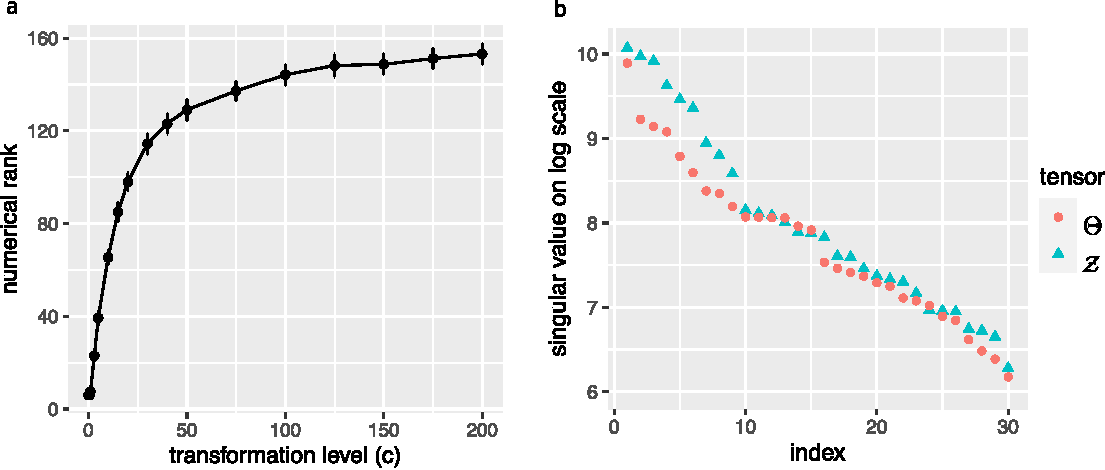
\includegraphics[width=.8\textwidth]{figure/example_comb.pdf}
 \captionsetup{justification=raggedright,font=small}
  \captionsetup{justification=raggedright,font=small}
\caption{(a) Numerical rank of $\Theta$ versus $c$ in the first example. (b) Top $d=30$ tensor singular values in the second example. }\label{fig:example}
\end{figure}
\vspace{-.7cm}

The second example demonstrates the inadequacy of classical low-rankness in representing special structures.  We consider the signal tensor of the form $\Theta=\log(1+\tZ)$, where $\tZ\in\mathbb{R}^{d\times d\times d}$ is an order-3 tensor with entries $\tZ(i,j,k)={1\over d}\max(i,j,k)$ for $i,j,k\in\{1,\ldots,d\}$. The matrix analogy of $\Theta$ was studied by~\cite{chan2014consistent} in graphon analysis. In this case neither $\Theta$ nor $\tZ$ is low-rank; in fact, the rank is no smaller than the dimension $d$ as illustrated in Figure~\ref{fig:example}b. Again,  the  low-rank models fail to address this type of tensor structure. 

In the above and many other examples, the signal tensors $\Theta$ of interest have high rank. Classical low-rank models will miss these important structures. New methods that allow flexible tensor modeling have yet to be developed. 


\subsection{Our contributions}
We develop a new model called sign representable tensors to address the aforementioned challenges. 
Figure~\ref{fig:demo} illustrates our main idea. Our approach is built on the sign series representation of the signal tensor, and we propose to estimate the sign tensors through a series of weighted classifications. In contrast to existing methods, our method is guaranteed to recover a wide range of low- and high-rank signals. We highlight two main contributions that set our work apart from earlier literature. 

\begin{figure}[h!]
\centerline{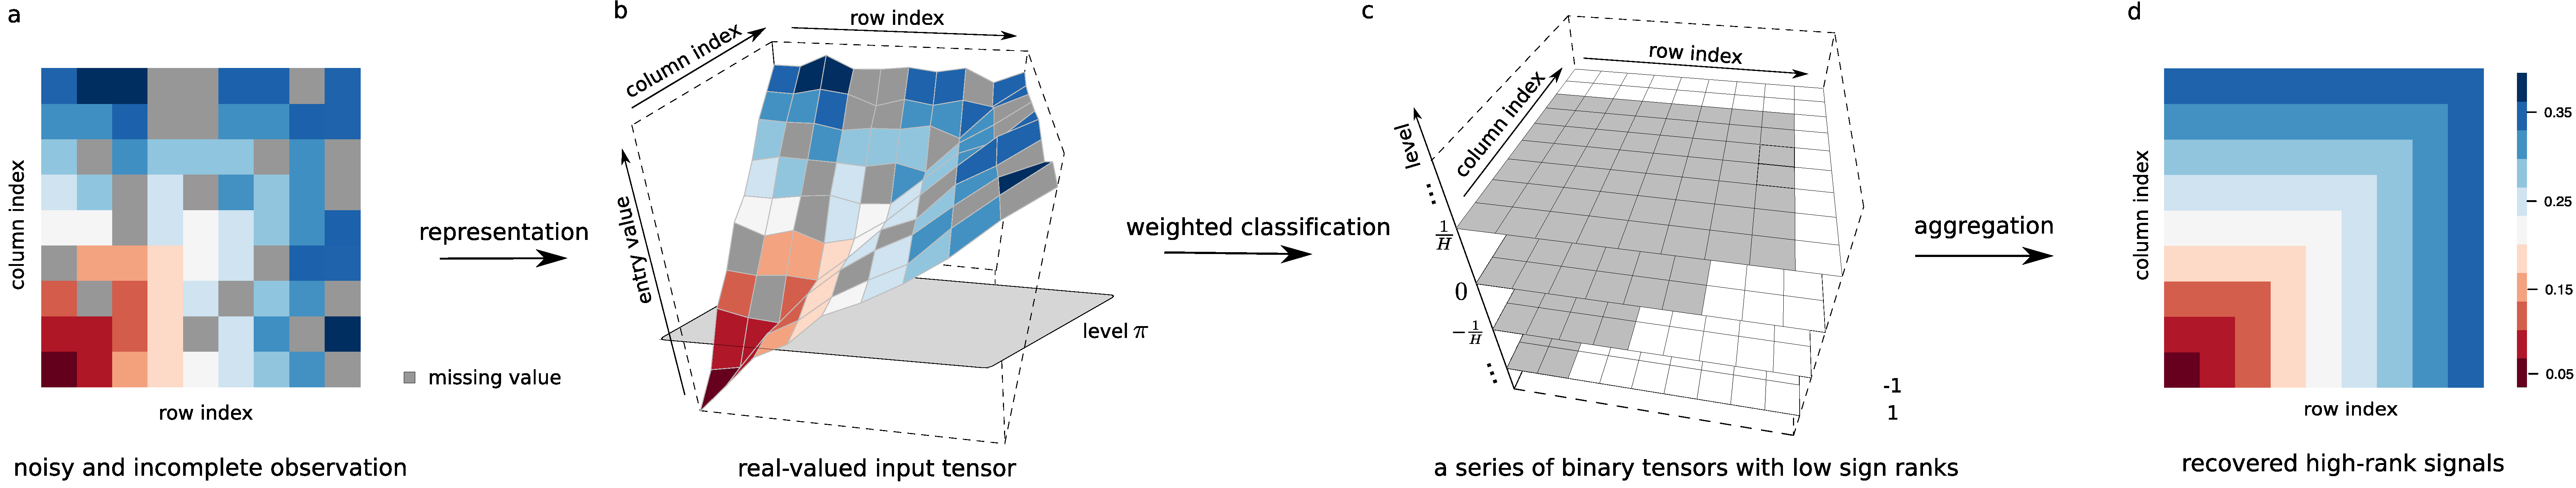
\includegraphics[width=1\textwidth]{figure/demo.pdf}}
 \captionsetup{justification=raggedright,font=small}
\caption{Illustration of our method. For visualization purpose, we plot an order-2 tensor (a.k.a.\ matrix); similar procedure applies to higher-order tensors. (a): a noisy and incomplete tensor input. (b) and (c): main steps of estimating sign tensor series $\sign(\Theta-\pi)$ for $\pi\in  \{-1,\ldots,-{1\over H},0,{1\over H},\ldots,1\}$. (d) estimated signal $\hat \Theta$. The depicted signal is a full-rank matrix based on Example~\ref{eq:example} in Section~\ref{sec:representation}.}\label{fig:demo}
\end{figure}
\vspace{-.3cm}

Statistically, the problem of high-rank tensor estimation is challenging. Existing estimation theory~\citep{anandkumar2014tensor,montanari2018spectral,cai2019nonconvex} exclusively focuses on the regime of fixed $r$ growing $d$. However, such premise fails in high-rank tensors, where the rank may grow with, or even exceed, the dimension. A proper notion of nonparametric complexity is crucial. We show that the sign tensor series not only preserves all information in the original signals, but also brings the benefits of flexibility and accuracy over classical low-rank models. The results fill the gap between parametric (low-rank) and nonparametric (high-rank) tensors, thereby greatly enriching the tensor model literature. 

From computational perspective, optimizations regarding tensors are in general NP-hard. Fortunately, tensors sought in applications are specially-structured, for which a number of efficient algorithms are available~\citep{ghadermarzy2018learning,wang2018learning, han2020optimal}. Our high-rank tensor estimate is provably reductable to a series of classifications, and its divide-and-conquer nature facilitates efficient computation. The ability to import and adapt existing tensor algorithms is one advantage of our method. 

We also highlight the challenges associated with tensors compared to matrices. High-rank matrix estimation is recently studied under nonlinear models~\citep{ganti2015matrix} and subspace clustering~\citep{pmlr-v70-ongie17a,fan2019online}. However, the problem for high-rank tensors is more challenging, because the tensor rank often exceeds the dimension when order $K\geq 3$~\citep{anandkumar2017analyzing}.  We show that, applying matrix methods to higher-order tensors results in suboptimal estimates. A full exploitation of the higher-order structure is needed; this is another challenge we address in this paper.

\vspace{-.3cm}
\subsection{Notation}
We use $\sign(\cdot)\colon \mathbb{R}\to\{-1,1\}$ to denote the sign function, where $\sign(y)=1$ if $y\geq 0$ and $-1$ otherwise. We allow univariate functions, such as $\sign(\cdot)$ and general $f\colon \mathbb{R}\to\mathbb{R}$, to be applied to tensors in an element-wise manner. 
We denote $a_n\lesssim b_n$ if $\lim_{n\to \infty} a_n/b_n\leq c$ for some constant $c\geq0$.  We use the shorthand $[n]$ to denote the $n$-set $\{1,\ldots,n\}$ for $n\in\mathbb{N}_{+}$. Let $\Theta\in\mathbb{R}^{d_1\times \cdots \times d_K}$ denote an order-$K$ $(d_1,\ldots,d_K)$-dimensional tensor, and $\Theta(\omega)\in\mathbb{R}$ denote the tensor entry indexed by $\omega \in[d_1]\times \cdots \times [d_K]$. An event $E$ is said to occur ``with very high probability'' if $\mathbb{P}(E)$ tends to 1 faster than any polynomial of tensor dimension $d:=\min_k d_k \to\infty$. The CP decomposition~\citep{hitchcock1927expression} is defined by
\begin{equation}\label{eq:CP}
\Theta=\sum_{s=1}^r\lambda_s \ma^{(1)}_s\otimes\cdots\otimes \ma^{(K)}_s,
\end{equation}
where $\lambda_1\geq \cdots \geq \lambda_r>0$ are tensor singular values, $\ma^{(k)}_s\in\mathbb{R}^{d_k}$ are norm-1 tensor singular vectors, and $\otimes$ denotes the outer product of vectors. The minimal $r\in\mathbb{N}_{+}$ for which~\eqref{eq:CP} holds is called the tensor rank, denoted $\rank(\Theta)$.  

\vspace{-.5cm}
\section{Model and proposal overview}\label{sec:overview}
Let $\tY$ be an order-$K$ $(d_1,\ldots,d_K)$-dimensional data tensor generated from the  model,
\begin{equation}\label{eq:model}
\tY=\Theta+\tE,
\end{equation}
where $\Theta\in\mathbb{R}^{d_1\times \cdots \times d_K}$ is an unknown signal tensor of interest, and $\tE$ is a noise tensor consisting of zero-mean, independently but not necessarily identically distributed entries. We allow heterogenous noise, in that the marginal distribution of noise entry $\tE(\omega)$ may depend on $\omega$. For simplicity, we assume the noise is bounded; the extension to a sub-Gaussian noise is provided in Appendix (omitted in current version). In the main paper we assume the range of $\tY$ is the bounded interval $[-1,1]$ for cleaner exposition.

Our observation is an incomplete data tensor from~\eqref{eq:model}, denoted  $\tY_\Omega$, where $\Omega\subset[d_1]\times\cdots\times[d_K]$ is the index set of observed entries. We consider a general model on $\Omega$ that allows both uniform and non-uniform samplings. Specifically, let $\Pi=\{p_\omega\}$ be an arbitrarily predefined probability distribution over the full index set with $\sum_{\omega\in[d_1]\times \cdots \times [d_K]}p_\omega=1$. Assume that the entries $\omega$ in $\Omega$ are i.i.d.\ draws with replacement from the full index set using distribution $\Pi$. 

Before describing our main results, we provide the intuition behind our method. In the two examples in Section~\ref{sec:intro}, the high-rankness in the signal $\Theta$ makes the estimation challenging. Let us examine the sign of the $\pi$-shifted signal $\sign(\Theta-\pi)$ for any given $\pi\in[-1,1]$. It turns out that these sign tensors share the same sign patterns as low-rank tensors. Indeed, the signal tensor in the first example has the same sign pattern as a rank-$4$ tensor, since $\sign(\Theta-\pi)=\sign(\tZ-f^{-1}(\pi))$. The signal tensor in the second example has the same sign pattern as a rank-2 tensor (see Example~\ref{eq:example} in Section~\ref{sec:representation}).


The above observation suggests a general framework to estimate both low- and high-rank signal tensors. Figure~\ref{fig:demo} illustrates the main crux of our method. We dichotomize the data tensor into a series of sign tensors $\sign (\tY_\Omega-\pi)$ for $\pi\in \tH={\{\small-1,\ldots,  -{1\over H},0, {1\over H},\ldots,1\}}$. Then, we estimate the sign signals $\sign(\Theta-\pi)$ by performing classification
\[
\hat \tZ_\pi=\argmin_{\text{low rank tensor $\tZ$}} \text{Weighted-Loss}(\sign(\tZ), \sign (\tY_\Omega-\pi)),
\]
where Weighted-Loss$(\cdot,\cdot)$ denotes a carefully-designed classification objective function which will be described in later sections. Our final proposed tensor estimate takes the form
\vspace{-.5cm}
\[
\hat \Theta = {1\over 2H+1}\sum_{\pi \in \tH} \sign(\hat \tZ_\pi).
\]
Our approach is built on the nonparametric sign representation of signal tensors. The estimate $\hat \Theta$ is essentially learned from dichotomized tensor series $\{\sign(\tY_\Omega-\pi)\colon \pi \in \tH\}$ with proper weights. We show that a careful aggregation of dichotomized data not only preserves all information in the original signals, but also brings benefits of accuracy and flexibility over classical low-rank models. Unlike traditional methods, the sign representation is guaranteed to recover both low- and high-rank signals that were previously impossible. The method enjoys statistical effectiveness and computational efficiency. 

\vspace{-.3cm}

\section{Statistical properties of sign representable tensors}\label{sec:representation}
This section develops sign representable tensor models for $\Theta$ in~\eqref{eq:model}. We characterize the algebraic and statistical properties of sign tensor series, which serves our theoretical foundation. 

\vspace{-.2cm}

\subsection{Sign-rank and sign tensor series}\label{sec:sign-rank}
Let $\Theta$ be the tensor of interest, and $\sign (\Theta)$ the corresponding sign pattern. The sign patterns induce an equivalence relationship between tensors. Two tensors are called sign equivalent, denoted $\simeq$, if they have the same sign pattern.

\vspace{-.3cm}

\begin{defn}[Sign-rank]
The sign-rank of a tensor $\Theta\in\mathbb{R}^{d_1\times \cdots \times d_K}$ is defined by the minimal rank among all tensors that share the same sign pattern as $\Theta$; i.e.,
\[
\srank(\Theta) = \min \{\rank(\Theta')\colon  \Theta'\simeq \Theta,\ \Theta'\in\mathbb{R}^{d_1\times \cdots \times d_K}\}.
\]
\end{defn}
The sign-rank is also called support rank~\citep{cohn2013fast}, minimal rank~\citep{alon2016sign}, and nondeterministic rank~\citep{de2003nondeterministic}. Earlier work defines sign-rank for binary-valued tensors; we extend the notion to continuous-valued tensors. Note that the sign-rank concerns only the sign pattern but discards the magnitude information of $\Theta$. In particular, $\srank(\Theta)=\srank(\sign \Theta)$. 

Like most tensor problems~\citep{hillar2013most}, determining the sign-rank for a general tensor is NP hard~\citep{alon2016sign}. Fortunately, tensors arisen in applications often possess special structures that facilitate analysis. By definition, the sign-rank is upper bounded by the tensor rank. More generally, we have the following upper bounds. 

\vspace{-.3cm}

\begin{prop}[Upper bounds of the sign-rank]~\label{cor:monotonic} For any strictly monotonic function $g\colon \mathbb{R}\to \mathbb{R}$ with $g(0)=0$, we have $\textup{srank}(\Theta)\leq\rank(g(\Theta))$.
\end{prop}

Conversely, the sign-rank can be much smaller than the tensor rank as shown earlier. 

\begin{prop}[Broadness]\label{prop:extention}\label{cor:broadness}For every order $K\geq 2$ and dimension $d$, there exist tensors $\Theta\in\mathbb{R}^{d\times \cdots \times d}$ such that $\rank(\Theta)\geq d$ but $\srank(\Theta-\pi)\leq 2$ for all $\pi\in\mathbb{R}$.  
\end{prop}
The two examples in Section~\ref{sec:intro} fall into this category where tensor rank grows with dimension $d$ but the sign-rank remains a constant. The results highlight the advantages of using sign-rank in the high-dimensional tensor analysis. Propositions~\ref{cor:monotonic} and~\ref{prop:extention} together demonstrate the strict broadness of low sign-rank family over the usual low-rank family. 

We now introduce  ``sign representable tensors'' for the signal model in \eqref{eq:model}.
\vspace{-.3cm}

\begin{defn}[Sign representable tensors] 
Fix a level $\pi\in[-1,1]$. A tensor $\Theta$ is called $(r,\pi)$-sign representable, if the tensor $(\Theta-\pi)$ has sign-rank bounded by $r$. A tensor $\Theta$ is called $r$-sign (globally) representable, if $\Theta$ is $(r,\pi)$-sign representable for all $\pi\in[-1,1]$. The collection $\{\sign(\Theta-\pi)\colon \pi \in[-1,1]\}$ is called the sign tensor series. 
We use $\caliP(r)=\{\Theta\colon \max_{\pi\in[-1,1]}\srank(\Theta-\pi)\leq r\}$ to denote the $r$-sign representable tensor family.
\end{defn}

We show that the $r$-sign representable tensor family is a general model that incorporates most existing tensor models, including low-rank tensors, single index models, GLM models, and several hypergraphon models. 
\vspace{-.3cm}

\begin{example}[CP/Tucker low-rank models] The CP and Tucker low-rank tensors are the two most popular tensor models~\citep{kolda2009tensor}. Let $\Theta$ be a low-rank tensor with CP rank $r$. We see that $\Theta$ belongs to the sign representable family; i.e., $\Theta\in\caliP(r+1)$ (the constant $1$ is due to $\rank(\Theta-\pi)\leq r+1$). Similar results hold for Tucker low-rank tensors $\Theta\in\caliP(r+1)$, where $r=\prod_kr_k$ with $r_k$ being the $k$-th mode Tucker rank of $\Theta$.  
\end{example} 
\vspace{-.3cm}

\begin{example}[Tensor block models (TBMs)] Tensor block model~\citep{wang2019multiway,chi2020provable} assumes a checkerboard structure among tensor entries under marginal index permutation. The signal tensor $\Theta$ takes at most $r$ distinct values, where $r$ is the total number of multiway blocks. Our model incorporates TBM because $\Theta \in \caliP(r)$. 
\end{example}
\vspace{-.3cm}


\begin{example}[Generalized linear models (GLMs)] Let $\tY$ be a binary tensor from a logistic model~\citep{wang2018learning} with mean $\Theta=\text{logit}(\tZ)$, where $\tZ$ is a latent low-rank tensor. Notice that $\Theta$ itself may be high-rank (see Section~\ref{sec:intro}). By definition, $\Theta$ is a low-rank sign representable tensor. Same conclusion holds for general exponential-family models with a (known) link function~\citep{hong2020generalized}. 
\end{example}
\vspace{-.3cm}

\begin{example}[Single index models (SIMs)] Single index model is a flexible semiparametric model proposed in economics~\citep{robinson1988root} and high-dimensional statistics~\citep{balabdaoui2019least,ganti2017learning}. We here extend the model to higher-order tensors $\Theta$. The SIM assumes the existence of a (unknown) monotonic function $g\colon \mathbb{R}\to \mathbb{R}$ such that $g(\Theta)$ has rank $r$. We see that $\Theta$ belongs to the sign representable family; i.e., $\Theta\in \caliP(r+1)$. 
\end{example}
\vspace{-.3cm}

\begin{example}[Min/Max hypergraphon]\label{eq:example}Graphon is a popular nonparametric model for networks~\citep{chan2014consistent,xu2018rates}. Here we revisit the model introduced in Section~\ref{sec:intro} for generality. Let $\Theta$ be an order-$K$ tensor generated from the hypergraphon $\Theta(i_1,\ldots,i_K)=\log(1+\max_kx^{(k)}_{i_k})$, where $x^{(k)}_{i_k}$ are given number in $[0,1]$ for all $i_k\in[d_k], k\in[K]$. We conclude that $\Theta \in \caliP(2)$, because the sign tensor $\sign(\Theta-\pi)$ with an arbitrary $\pi\in(0,\ \log 2)$ is a block tensor with at most two blocks (see Figure~\ref{fig:demo}c).

The results extend to general min/max hypergraphons. Let $g(\cdot)$ be a continuous univariate function with at most $r\geq 1$ distinct real roots in the equation $g(z)=\pi$; e.g., when $g(z)$ is a polynomial of degree $r$. Then, the tensor $\Theta$ generated from $\Theta(i_1,\ldots,i_K)=g(\max_kx^{(k)}_{i_k})$ belongs to $\caliP(2r)$. Same conclusion holds if the maximum is replaced by the minimum. 
\end{example}

\vspace{-.6cm}
\subsection{Statistical characterization of sign tensors via weighted classification}\label{sec:identifiability}

Accurate estimation of a sign representable tensor depends on the behavior of sign tensor series, $\sign(\Theta-\pi)$. In this section, we show that sign tensors are completely characterized by weighted classification. The results bridge the algebraic and statistical properties of sign representable tensors.
 
For a given $\pi \in [-1,1]$, define a $\pi$-shifted data tensor $\bar \tY_\Omega$ with entries $\bar \tY(\omega) = (\tY(\omega)-\pi)$ for $\omega\in \Omega$. We propose a weighted classification objective function
\begin{equation}\label{eq:sample}
L(\tZ, \bar \tY_\Omega)= {1\over |\Omega|}\sum_{\omega \in \Omega}\ \KeepStyleUnderBrace{|\bar \tY(\omega)|}_{\text{weight}}\  \times \ \KeepStyleUnderBrace{| \sign \tZ(\omega)-\sign \bar \tY(\omega)|}_{\text{classification loss}},
\end{equation}
where $\tZ\in\mathbb{R}^{d_1\times \cdots \times d_K}$ is the decision variable to be optimized, $|\bar \tY(\omega)|$ is the entry-specific weight equal to the distance from the tensor entry to the target level $\pi$. The entry-specific weights incorporate the magnitude information into classification, where entries far away from the target level are penalized more heavily in the objective. In the special case of binary tensor $\tY\in\{-1,1\}^{d_1\times\cdots\times d_K}$ and target level $\pi=0$, the loss~\eqref{eq:sample} reduces to usual classification loss.
Our proposed weighted classification function~\eqref{eq:sample} is important for characterizing $\sign(\Theta-\pi)$. Define the weighted classification risk 
\begin{equation}\label{eq:population}
\textup{Risk}(\tZ)=\mathbb{E}_{\tY_\Omega}L(\tZ,\bar\tY_\Omega),
\end{equation}
where the expectation is taken with respect to $\tY_\Omega$ under model~\eqref{eq:model} and the sampling distribution $\omega\sim\Pi$. Note that the form of $\textup{Risk}(\cdot)$ implicitly depends on $\pi$; we suppress $\pi$ when no confusion arises. 

\vspace{-.3cm}

\begin{prop}[Global optimum of weighted risk]\label{prop:global}
Suppose the data $\tY_\Omega$ is generated from model~\eqref{eq:model} with $\Theta \in \caliP(r)$. Then, for all $\bar \Theta$ that are sign equivalent to $\sign(\Theta-\pi)$, 
\begin{align}\label{eq:optimal}
\textup{Risk}(\bar \Theta )&=\inf\{\textup{Risk}(\tZ)\colon \tZ\in\mathbb{R}^{d_1\times \cdots \times d_K}\}
=\inf\{\textup{Risk}(\tZ)\colon \textup{rank} (\tZ)\leq r\}.
\end{align}
\end{prop}
The results show that the sign tensor $\sign(\Theta-\pi)$ optimizes the weighted classification risk. This fact suggests a practical procedure to estimate $\sign(\Theta-\pi)$ via empirical risk optimization of $L(\tZ,\bar \tY_\Omega)$. In order to establish the recovery guarantee, we shall address the uniqueness (up to sign equivalence) for the optimizer of $\risk(\cdot)$. The local behavior of $\Theta$ around $\pi$ turns out to play a key role in the accuracy. 

Some additional notation is needed for stating the results in full generality. Let $d_t=\prod^K_{k=1} d_k$ denote the total number of tensor entries, and $\Delta s = 2/d_t$ a small tolerance. We quantify distribution of entries in tensor $\Theta$ using pseudo density (a.k.a. histogram with bin width $\Delta s$). Specifically, let $G(\pi):=\mathbb{P}_{\omega\sim \Pi}[\Theta(\omega)\leq \pi]$ denote the cumulative distribution function (CDF) of $\Theta(\omega)$ under $\omega\sim \Pi$. We partition $[-1,1]=\tN \cup \tN^c$, where $\tN$ consists of levels whose pseudo density based on $\Delta s$-bin is asymptotically unbounded; i.e,
\[
\tN=\left\{\pi\in[-1,1] \colon {G(\pi+{\Delta s/2})-G(\pi-{\Delta s/2})\over \Delta s} \geq C \right\},\ \text{for some universal constant }C>0,
\]
and $\tN^c$ otherwise. 
Note that both $\Theta$ and its induced CDF $G$ implicitly depend on the tensor dimension. We impose assumptions to $G=G_d$ in the high-dimensional regime uniformly as $d:=\min_k d_k \to\infty$. 

\begin{assumption}[$\alpha$-smoothness]\label{ass:margin} Fix $\pi \notin \tN$. Assume there exist constants $\alpha=\alpha(\pi)> 0, c=c(\pi) >0$, independent of tensor dimension, such that, 
\begin{equation}\label{eq:smooth}
\sup_{\Delta s \leq t<\rho(\pi, \tN)}{G(\pi+{t/2})-G(\pi-{t/2})\over t^\alpha} \leq c,
\end{equation}
where $\rho(\pi,\tN):=\min_{\pi'\in \tN}|\pi-\pi'|$ denotes the distance from $\pi$ to the nearest point in $\tN$. The largest possible $\alpha=\alpha(\pi)$ in~\eqref{eq:smooth} is called the smoothness index at level $\pi$. We make the convention that $\alpha=\infty$ if the numerator in~\eqref{eq:smooth} is zero, implying almost no entries of $\Theta(\omega)$ around the level $\pi$. We call a tensor $\Theta$ is $\alpha$-globally smooth, if~\eqref{eq:smooth} holds with global constants $\alpha>0, c>0$ for all $\pi\notin\tN$. 
\end{assumption}

The smoothness index $\alpha$ quantifies the intrinsic hardness of recovering $\sign(\Theta-\pi)$ from $\risk(\cdot)$. 
The value of $\alpha$ depends on both the sampling distribution $\omega\sim \Pi$ and the behavior of $\Theta(\omega)$. 
The recovery is easier at levels where points are less concentrated around $\pi$ with a large value of $\alpha>1$, or equivalently, when $G(\pi)$ remains almost  flat around $\pi$. A small value of $\alpha<1$ indicates the nonexistent (infinite) density at level $\pi$, or equivalently, when the $G(\pi)$ jumps by greater than the tolerance $\Delta s$ at $\pi$. Fig~\ref{fig:demo} illustrates three examples of $G(\pi)$. 

\begin{figure}
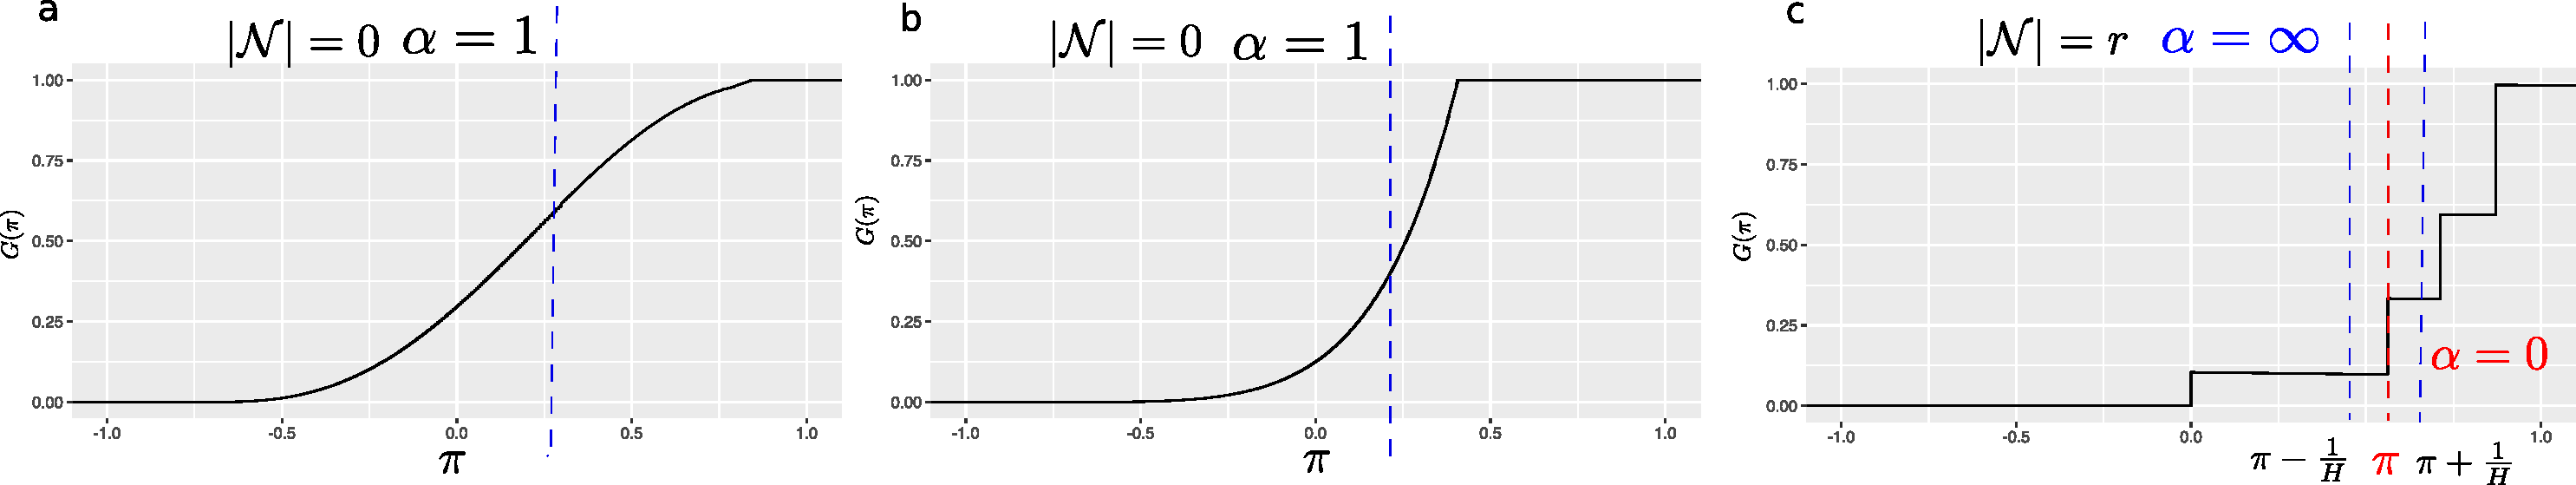
\includegraphics[width=.95\textwidth]{figure/cdf_new.pdf}
\captionsetup{justification=raggedright,font=small}
\caption{Three examples of CDF, $G(\pi)=\mathbb{P}_{\mX}(f(\mX)\leq \pi)$, and the associated smoothness index $\alpha$. (a) and (b) $G(\pi)$ with $\alpha=1$ because the function $G(\pi)$ induces bounded pseudo density in the range of $\pi$. (c) $G(\pi)$ with $\alpha=\infty$ at most $\pi$ (in blue) except for a few jump points with $\alpha=0$ (in red). The dashed lines correspond to local $(\alpha,\pi)$-smoothness.}\label{fig:demo}
\label{fig:CDF}
\end{figure}

We now reach the main theorem in this section. For two tensors $\Theta_1,\Theta_2$, define the mean absolute error (MAE) as
$\text{MAE}(\Theta_1, \Theta_2)\stackrel{\text{def}}{=}\mathbb{E}_{\omega\sim \Pi}|\Theta_1(\omega)-\Theta_2(\omega)|.$


\begin{thm}[Identifiability]\label{thm:population}Under Assumption~\ref{ass:margin}, for all tensors $\bar \Theta \simeq \sign(\Theta-\pi)$ and tensors $\tZ\in\mathbb{R}^{d_1\times \cdots \times d_K}$,
\[
\textup{MAE}(\sign \tZ, \sign \bar \Theta) \leq C(\pi)\left[\textup{Risk}(\tZ)-\textup{Risk}( \bar \Theta)\right]^{\alpha/(\alpha+1)},
\]
where $C(\pi)>0$ is independent of $\tZ$. 
\end{thm}
The result establishes the recovery stability of sign tensors $\sign (\Theta-\pi)$ using optimization with population risk~\eqref{eq:population}. The bound immediately shows the uniqueness of the optimizer  for $\text{Risk}(\cdot)$ up to a zero-measure set under $\Pi$. We find that a higher value of $\alpha$ implies more stable recovery, as intuition would suggest. Similar results hold for optimization with sample risk~\eqref{eq:sample} (see Section~\ref{sec:estimation}). 

We conclude this section by applying Assumption~\ref{ass:margin} to the examples described in Section~\ref{sec:sign-rank}. For simplicity, suppose $\Pi$ is the uniform sampling. 
The tensor block model is $\infty$-globally smooth. This is because the set $\tN$ consists of finite $\Delta s$-bin's covering the distinct block means in $\Theta$. Furthermore, we have $\alpha= \infty$ for all $\pi \notin \tN$, since the numerator in~\eqref{eq:smooth} is zero.  Similarly, the min/max hypergaphon model such that  $\Theta(i_1,\ldots,i_K) = \log(1+\max_{\ell = 1,\ldots K}i_\ell/d)$ is $\infty$-globally smooth because $\alpha=\infty$ for all $\pi$ except those in $\tN$, where $\tN$ collects $d$ many $\Delta s$-bin's covering $\log(1+i/d)$ for $i =1,\ldots, d$.


\vspace{-.5cm}

\section{Nonparametric tensor completion via sign series}\label{sec:estimation}
In previous sections we have established the sign series representation and its relationship to classification. Now, we present our algorithm proposed in Section~\ref{sec:overview} in details. We provide the estimation error bound and address the empirical implementation of the algorithm. 
\vspace{-.3cm}

\subsection{Estimation error and sample complexity}

Given a noisy incomplete tensor observation $\tY_\Omega$ from model~\eqref{eq:model}, we cast the problem of estimating $\Theta$ into a series of weighted classifications. Specifically we propose the tensor estimate using the sign representation,
\begin{equation}\label{eq:est}
\hat \Theta = {1\over 2H+1}\sum_{\pi \in \tH}\sign{\hat \tZ_\pi},
\end{equation}
where, for each $\pi \in \tH=\{-1,\ldots,-{1\over H}, 0, {1\over H},\ldots,1\}$, the tensor $\hat \tZ_\pi\in\mathbb{R}^{d_1\times \dots\times d_K}$ is the $\pi$-weighted classifier estimated by
\begin{equation}\label{eq:estimate}
\hat \tZ_\pi = \argmin_{\tZ\colon \text{rank}\tZ\leq r} L(\tZ, \tY_\Omega-\pi).
\end{equation}
Here $L(\cdot,\cdot)$ denotes the weighted classification objective defined in~\eqref{eq:sample}, where we have plugged $\bar \tY_\Omega=(\tY_\Omega-\pi)$ in the expression, and the rank constraint follows from Proposition~\ref{prop:global}. For the theory, we assume the true $r$ is known; in practice, $r$ could be chosen in a data adaptive fashion via cross-validation or elbow method~\citep{hastie2009elements}. 

The next theorem establishes the statistical convergence for the sign tensor estimate~\eqref{eq:estimate}, which is an important ingredient for the final signal tensor estimate $\hat \Theta$ in~\eqref{eq:est}. 

\vspace{-.3cm}
 \begin{thm}[Sign tensor estimation]\label{thm:classification} Suppose $\Theta\in\caliP(r)$ and $\Theta(\omega)$ is $\alpha$-globally smooth under $\omega\sim \Pi$. Let $\hat \tZ_\pi$ be the estimate in~\eqref{eq:estimate}, $d_{\max}=\max_{k\in[K]} d_k$, and $d_{\max}r\lesssim |\Omega|$. Then, for all $\pi\in[-1,1]\setminus\tN$, with very high probability over $\tY_\Omega$, 
\begin{align}\label{eq:bound}
\textup{MAE}(\sign \hat \tZ_\pi, \sign(\Theta-\pi)) \lesssim  \left({d_{\max} r\over |\Omega|}\right)^{\alpha\over \alpha+2}+{1 \over \rho^2(\pi, \tN)} {d_{\max}r \over |\Omega|}.
\end{align}
\end{thm}
Theorem~\ref{thm:classification} provides the error bound for the sign tensor estimation. Compared to the population results in Theorem~\ref{thm:population}, we explicitly reveal the dependence of accuracy on the sample complexity and the level $\pi$. The result demonstrates the polynomial decay of sign errors with $|\Omega|$.  Our sign estimate achieves consistent recovery using as few as $\tilde O(d_{\max}r)$ noisy entries. 

Recall that $\tN$ collects the levels for which the sign tensor is possibly nonrecoverable. Let $|\tN|$ be the covering number of $\tN$ with $\Delta s$-bin's, i.e, $|\tN| = \lceil \mu(\tN)/\Delta s \rceil$, where $\mu$ is the Lebesgue measure. Combining the sign representability of the signal tensor and the sign estimation accuracy, we obtain the main results on our nonparametric tensor estimation method. 

\vspace{-.3cm}

\begin{thm}[Tensor estimation error]\label{thm:estimation} Consider the same conditions of Theorem~\ref{thm:classification}. Let $\hat \Theta$ be the estimate in~\eqref{eq:est} and $t_d={d_{\max}r /|\Omega|}$. With very high probability over $\tY_\Omega$,
\begin{equation}\label{eq:bound2}
\textup{MAE}(\hat \Theta, \Theta)\lesssim \left(t_d\right)^{\alpha/(\alpha+2)}+{1+|\tN|\over H}+{Ht_d}.
\end{equation}
In particular, setting $\scriptstyle H\asymp \left( (1+|\tN|)/ t_d \right)^{1/2}$ yields the error bound
\begin{equation}\label{eq:real}
\textup{MAE}(\hat \Theta, \Theta)\lesssim \max\left(t_d^{{2\alpha/ (\alpha+2)} },\ t_d(1+|\tN|)\right)^{1/2}.
\end{equation}
\end{thm}

Theorem~\ref{thm:estimation} demonstrates the convergence rate of our tensor estimation. The bound~\eqref{eq:bound2} reveals three sources of errors: the estimation error for sign tensors, the bias from sign series representations, and the variance thereof. The resolution parameter $H$ controls the bias-variance tradeoff. We remark that the signal estimation error~\eqref{eq:real} is generally no better than the corresponding sign error~\eqref{eq:bound}. This is to be expected, since magnitude estimation is  a harder problem than sign estimation. 

In the special case of full observation with equal dimension $d_k=d, k\in[K]$, our signal estimate achieves convergence
\begin{equation}
\textup{MAE}(\hat \Theta, \Theta)\lesssim\max\left( \left(rd^{-(K-1)}\right)^{2\alpha /( \alpha+2)},\ rd^{-(K-1)}(1+|\tN|)\right)^{1/2}.
\end{equation}
Compared to earlier methods, our estimation accuracy applies to both low- and high-rank signal tensors. The rate depends on the sign complexity $\Theta\in\caliP(r)$, and this $r$ is often much smaller than the usual tensor rank (see Section~\ref{sec:sign-rank}). Our result also reveals that the convergence becomes favorable as the order of data tensor increases. 

We apply our method to the main examples in Section~\ref{sec:sign-rank}, and compare the results with existing literature. The numerical comparison is provided in Section~\ref{sec:simulation}. 
\vspace{-.3cm}

\begin{customexample}{2}[TBMs]
Consider a tensor block model with $r$ multiway blocks. Our result implies a rate $\tO(d^{-(K-1)/2})$ by taking $\alpha=\infty$ and $|\tN| \leq r^K$. This rate agrees with the  previous root-mean-square error (RMSE) for block tensor estimation~\citep{wang2019multiway}.
\end{customexample}
\vspace{-.3cm}

\begin{customexample}{3} [GLMs] 
Consider a GLM tensor $\Theta=g(\tZ)$, where $g$ is a known link function and $\tZ$ is a latent low-rank tensor. Suppose the marginal density of $\Theta(\omega)$ is uniformly bounded as $d\to\infty$. Applying our results with $\alpha=1$ and $|\tN|<C$ for some constant $C>0$ yields $\tO(d^{-(K-1)/3})$. This rate is slightly slower than the parametric RMSE rate~\citep{zhang2018tensor,wang2018learning}. One possible reason is that our estimate remains valid for unknown $g$ and general high-rank tensors. The nonparametric rate is the price one has to pay for not knowing the form $\Theta=g(\tZ)$ as a priori. 
\end{customexample}

\begin{customexample}{4}[SIMs]
The earlier example has shown the nonparametric rate $\tO(d^{-(K-1)/3})$ when applying our method to single index tensor model. In the matrix case with $K=2$, our result yields a nonparametric rate $\tO(d^{-1/3})$, which is faster compared to the RMSE rate $\tO(d^{-1/4})$ obtained by \cite{ganti2015matrix}. 

\end{customexample}

\begin{customexample}{5}[Min/Max hypergraphon]
We consider a more general model than that in Section~\ref{sec:intro}. Consider a $r$-sign representable tensor $\Theta\in \caliP(r)$ with at most $d$ distinct entries with repetition pattern not necessarily $\tZ_{\max}$. Applying our results with $\alpha=\infty$ and $|\tN|=d$ yields the rate $\tO(d^{-(K-2)/2})$. Intuitively, the rate roughly reflects the total degree of freedom $d^2$, where the factor $d$ corresponds to the number of distinct entries, and the other factor $d$ corresponds to complexity in each sign tensor. 
\end{customexample}

The following sample complexity for nonparamtric tensor completion is a direct consequence of Theorem~\ref{thm:estimation}. 
\vspace{-.3cm}

\begin{cor}[Sample complexity for nonparametric completion] Under the same conditions of Theorem~\ref{thm:estimation} with $\alpha\neq 0$ and bounded $|\tN|$, with high probability over $\tY_\Omega$, 
\[
\textup{MAE}(\hat \Theta, \Theta)\to 0, \quad \text{as}\quad {|\Omega|\over {d_{\max}} r}\to \infty.
\]
\end{cor}
Our result improves earlier work~\citep{yuan2016tensor,ghadermarzy2019near,pmlr-v119-lee20i} by allowing both low- and high-rank signals. Interestingly, the sample requirements depend only on the sign complexity $r$ but not the nonparametric complexity $\alpha$. Note that $\tilde \tO(d_{\max}r)$ roughly matches the degree of freedom of sign tensors, suggesting the optimality of our sample requirements. 

\subsection{Numerical implementation}
This section addresses the practical implementation of our estimation~\eqref{eq:est} illustrated in Figure~\ref{fig:demo}. Our sign representation of the signal estimate $\hat \Theta$ is an average of $2H+1$ sign tensors, which can be solved in a divide-and-conquer fashion. Briefly, we estimate the sign tensors $\tZ_\pi$ (detailed in the next paragraph) for the series $\pi \in \tH$ through parallel implementation, and then we aggregate the results to yield the output. The estimate enjoys low computational cost similar to a single sign tensor estimation.  


For the sign tensor estimation~\eqref{eq:estimate}, the problem reduces to binary tensor decomposition with a weighted classification loss. A number of algorithms have been developed for this problem~\citep{ghadermarzy2018learning,wang2018learning,hong2020generalized}. We adopt similar ideas by tailoring the algorithms to our contexts.  Following the common practice in classification, we replace the binary loss $\ell(z,y)=|\sign z - \sign y|$ with a surrogate loss $F(m)$ using a continuous function of margin $m:=z\sign(y)$. Examples of large-margin loss are hinge loss $F(m) = (1-m)_+$, logistic loss $F(m) =\log(1+e^{-m})$, and nonconvex $\psi$-loss $F(m)=2\min(1,(1-m)_+)$ with $m_{+}=\max(m,0)$. Similar estimation properties hold under Fisher consistency of surrogate loss~\citep{bartlett2006convexity} and technical lemmas. 

\vspace{-.6cm}
\begin{figure}[h]
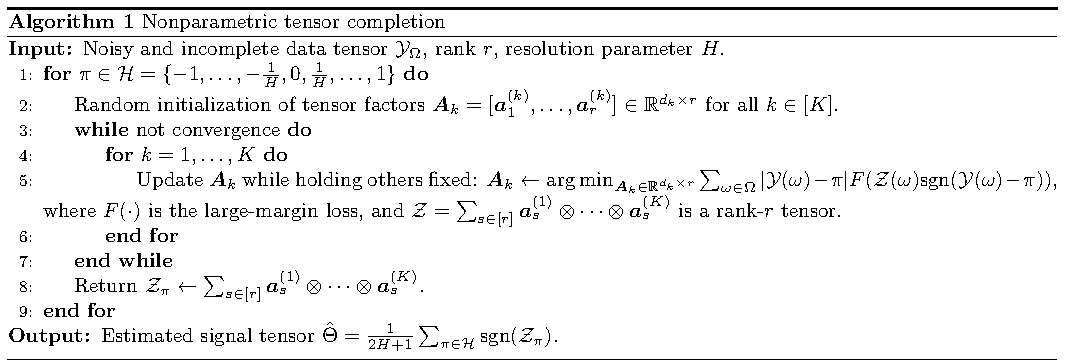
\includegraphics[width=\textwidth]{figure/algorithm.pdf}
\captionsetup{justification=raggedright,font=small}
\caption{The full procedure of algorithm for nonparametric tensor completion.}\label{fig:alg}
\end{figure}
\vspace{-2cm}
 
The rank constraints in the optimization~\eqref{eq:estimate} have been extensively studied in literature. Recent developments involve convex norm relaxation~\citep{ghadermarzy2018learning} and nonconvex optimization~\citep{wang2018learning, han2020optimal}. Unlike matrices, computing the tensor convex norm is NP hard, so we choose (non-convex) alternating optimization due to its numerical efficiency. Briefly, we use the rank decomposition~\eqref{eq:CP} of $\tZ=\tZ(\mA_1,\ldots, \mA_K)$ to optimize the unknown factor matrices $\mA_k=[\ma^{(k)}_1,\ldots,\ma^{(k)}_r]\in\mathbb{R}^{d_k\times r}$, where we choose to collect tensor singular values into $\mA_K$. We numerically solve \eqref{eq:est} by optimizing one factor $\mA_k$ at a time while holding others fixed. Each suboptimization reduces to a convex problem with a low-dimensional decision variable. Following common practice in tensor optimization~\citep{anandkumar2014tensor,hong2020generalized}, we implement  multiple initializations to locate a final estimate with the lowest objective value. Figure~\ref{fig:alg} describes the full procedure.

\section{Simulations}\label{sec:simulation}
In this section, we compare our nonparametric tensor method ({\bf NonParaT}) with two alternative approaches: low-rank tensor CP decomposition ({\bf CPT}), and the matrix version of our method applied to tensor unfolding ({\bf NonParaM}). We assess the performance under both complete and incomplete observations. The signal tensors are generated based on four models listed in Table~\ref{tab:simulation}. The simulation covers a wide range of complexity, including block tensors, transformed low rank tensors, min/max hypergraphon with logarithm and exponential functions. We consider order-3  tensors of equal dimension $d_1=d_2=d_3=d$, and set $d\in \{15, 20,\ldots,55,60\}$, $r=2$, $H=10+{(d-15)/ 5}$ in Algorithm 1. For {\bf NonParaM}, we apply Algorithm 1 to each of the three unfolded matrices and report the average error. All summary statistics are averaged across $30$ replicates.  

\begin{table}[h]
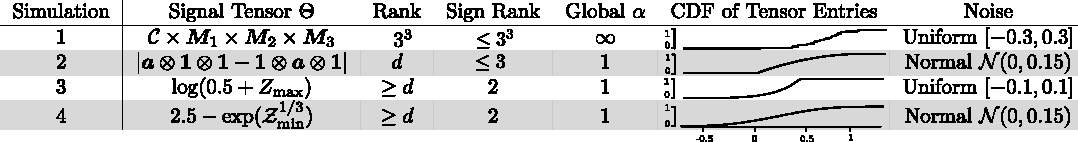
\includegraphics[width=1\textwidth]{figure/simulation.pdf}
 \captionsetup{justification=raggedright,font=small}
\caption{Simulation models used for comparison. We use $\mM_k\in\{0,1\}^{d\times 3}$ to denote membership matrices, $\tC\in\mathbb{R}^{3\times 3\times 3}$ the block means, $\ma={1\over d}(1,2,\ldots,d)^T \in\mathbb{R}^d$, $\tZ_{\max}$ and $\tZ_{\min}$ are order-3 tensors with entries ${1\over d}\max(i,j,k)$ and ${1\over d}\min(i,j,k)$, respectively.}\label{tab:simulation}
\end{table}
\vspace{-.5cm}

Figure~\ref{fig:compare1} compares the estimation error under full observation. The MAE decreases with tensor dimension for all three methods. We find that our method {\bf NonParaT} achieves the best performance in all scenarios, whereas the second best method is {\bf CPT} for models 1-2, and {\bf NonParaM} for models 3-4. One possible reason is that models 1-2 have controlled multilinear tensor rank, which makes tensor methods {\bf NonParaT} and {\bf CPT} more accurate than matrix methods. For models 3-4, the rank exceeds the tensor dimension. Therefore, the two nonparametric methods  exhibit the greater advantage for signal recovery. 



Figure~\ref{fig:compare2} shows the completion error against observation fraction. We fix $d=40$ and gradually increase the observation fraction ${|\Omega|\over d^3}$ from 0.3 to 1. We find that {\bf NonParaT} achieves the lowest error among all methods. Our simulation covers a reasonable range of  complexities; for example, model 1 has $3^3$ jumps in the CDF of signal $\Theta$, and models 2 and 4 have unbounded noise. Nevertheless, our method shows good performance in spite of model misspecification. This robustness is appealing in practice because the structure of underlying signal tensor is often unknown. 

\begin{figure}[h!]
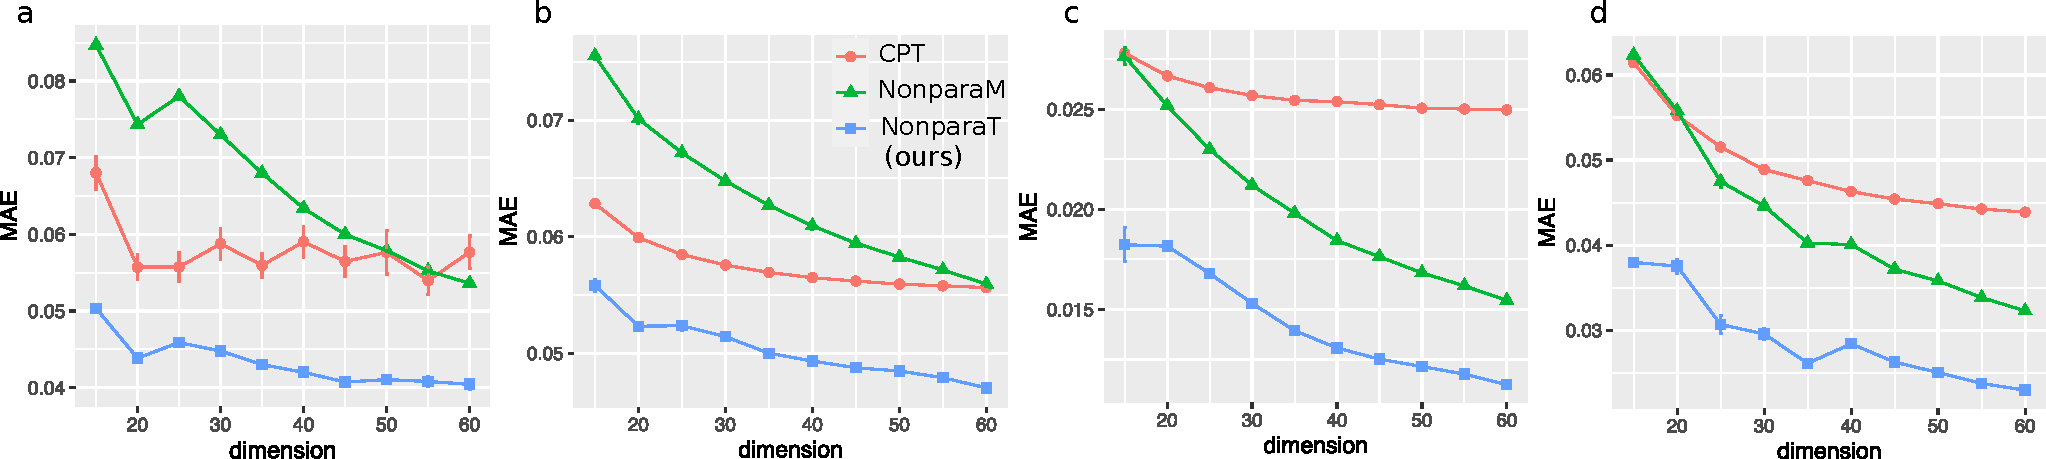
\includegraphics[width=\textwidth]{figure/fig1-4v2.pdf}
 \captionsetup{justification=raggedright,font=small}
\caption{Estimation error versus tensor dimension. Panels (a)-(d) correspond to simulation models 1-4 in Table~\ref{tab:simulation}.}\label{fig:compare1}
\end{figure}

\vspace{-.4cm}
\begin{figure}[h!]
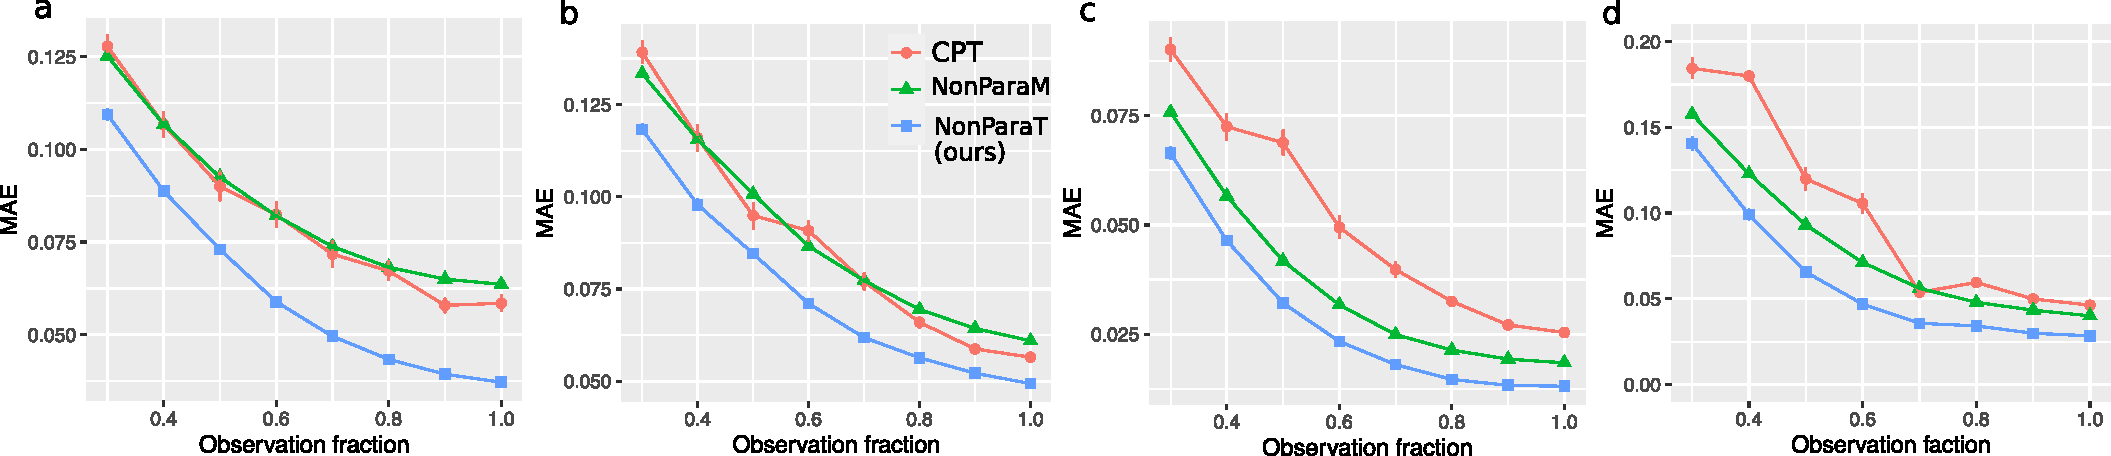
\includegraphics[width=\textwidth]{figure/fig5-8v2.pdf}
 \captionsetup{justification=raggedright,font=small}
\caption{Completion error versus observation fraction. Panels (a)-(d) correspond to simulation models 1-4 in Table~\ref{tab:simulation}. }\label{fig:compare2}
\end{figure}

\vspace{-1cm}

\section{Data applications}
We apply our method to two tensor datasets, the MRN-114 human brain connectivity data~\citep{wang2017bayesian}, and NIPS data~\citep{globerson2007euclidean}. The brain dataset records the structural connectivity among 68 brain regions for 114 individuals along with their Intelligence Quotient (IQ) scores. We organize the connectivity data into an order-3 tensor, where entries encode the presence or absence of fiber connections between brain regions across individuals. The NIPS dataset consists of word occurrence counts in papers published from 1987 to 2003. We focus on the top 100 authors, 200 most frequent words, and normalize each word count by log transformation with pseudo-count~1. The resulting dataset is an order-3 tensor with entry representing the log counts of words by authors across years. 





\begin{table}[h!]
\centering
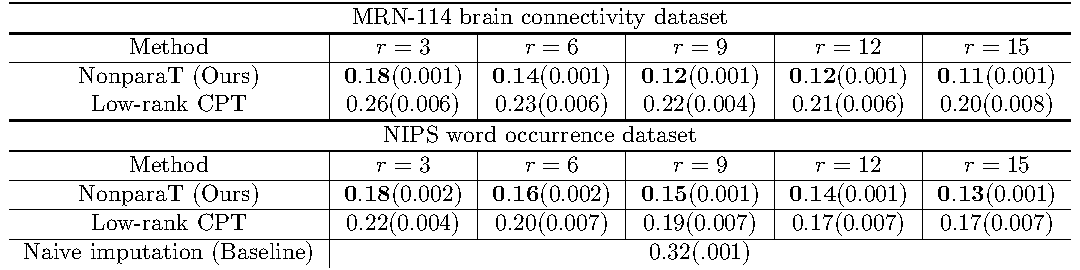
\includegraphics[width = \textwidth]{figure/table.pdf}
 \captionsetup{justification=raggedright,font=small}
\caption{MAE comparison in the brain data and NIPS data analysis. Reported MAEs are averaged over five runs of cross-validation, with 20\% entries for testing and 80\% for training, with standard errors in parentheses. Bold numbers indicate the minimal MAE among three methods. For low-rank CPT, we use R function {\tt rTensor} with default hyperparameters, and for our method, we set $H=20$.}\label{tab:data}
\end{table}
\vspace{-.4cm}

Table~\ref{tab:data} compares the prediction accuracy of different methods. Reported MAEs are averaged over five runs of cross-validation, with 20\% entries for testing and 80\% for training. Our method substantially outperforms the low-rank CP method for every configuration under consideration. Further increment of rank appears to have little effect on the performance, and we find that increased missingness gives more advantages to our method. The comparison highlights the advantage of our method in achieving accuracy while maintaining low complexity. 

\begin{figure}[h!]
\centering
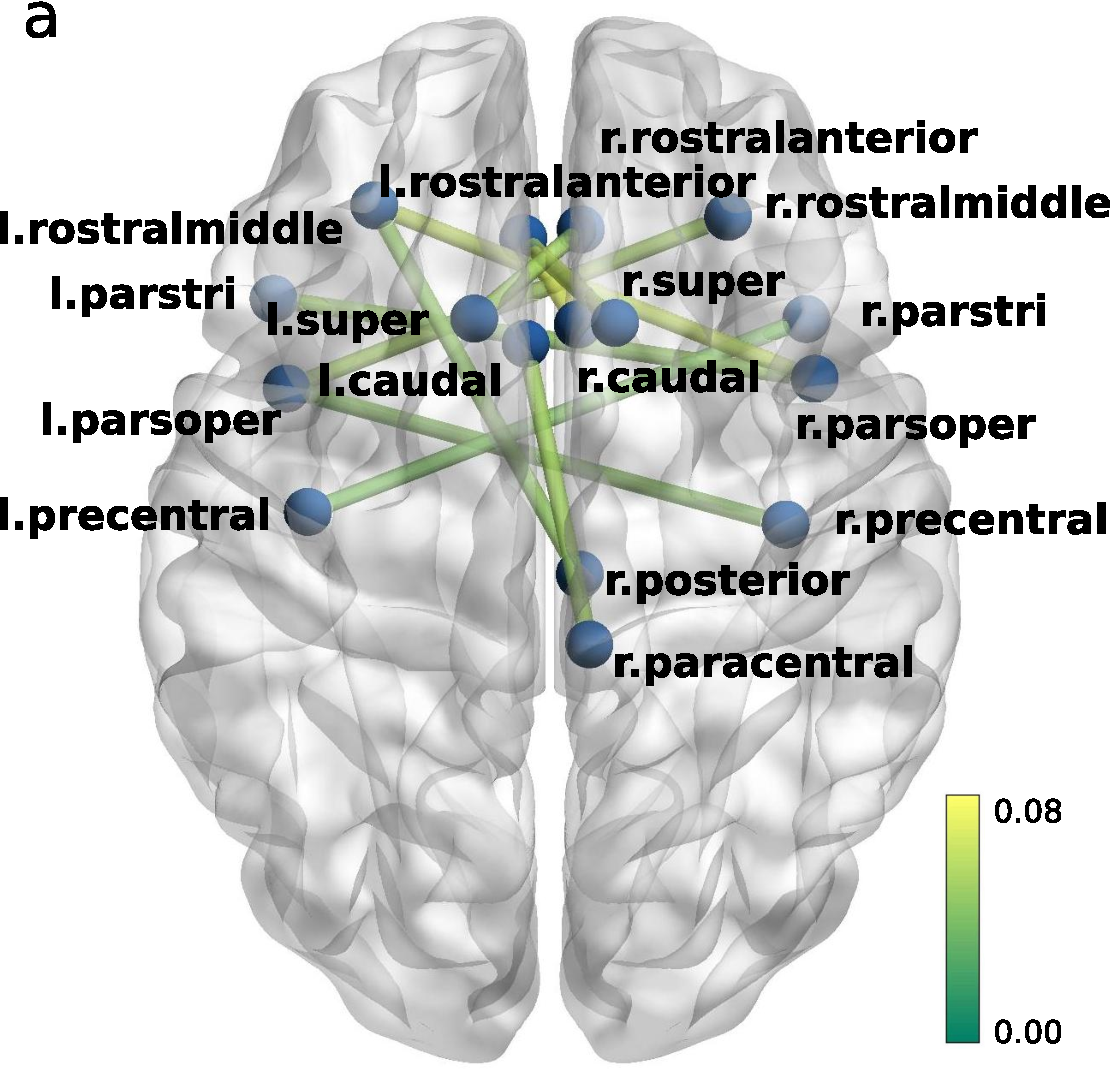
\includegraphics[width=.36\textwidth]{figure/brainIQ.pdf}
\hspace{1cm}
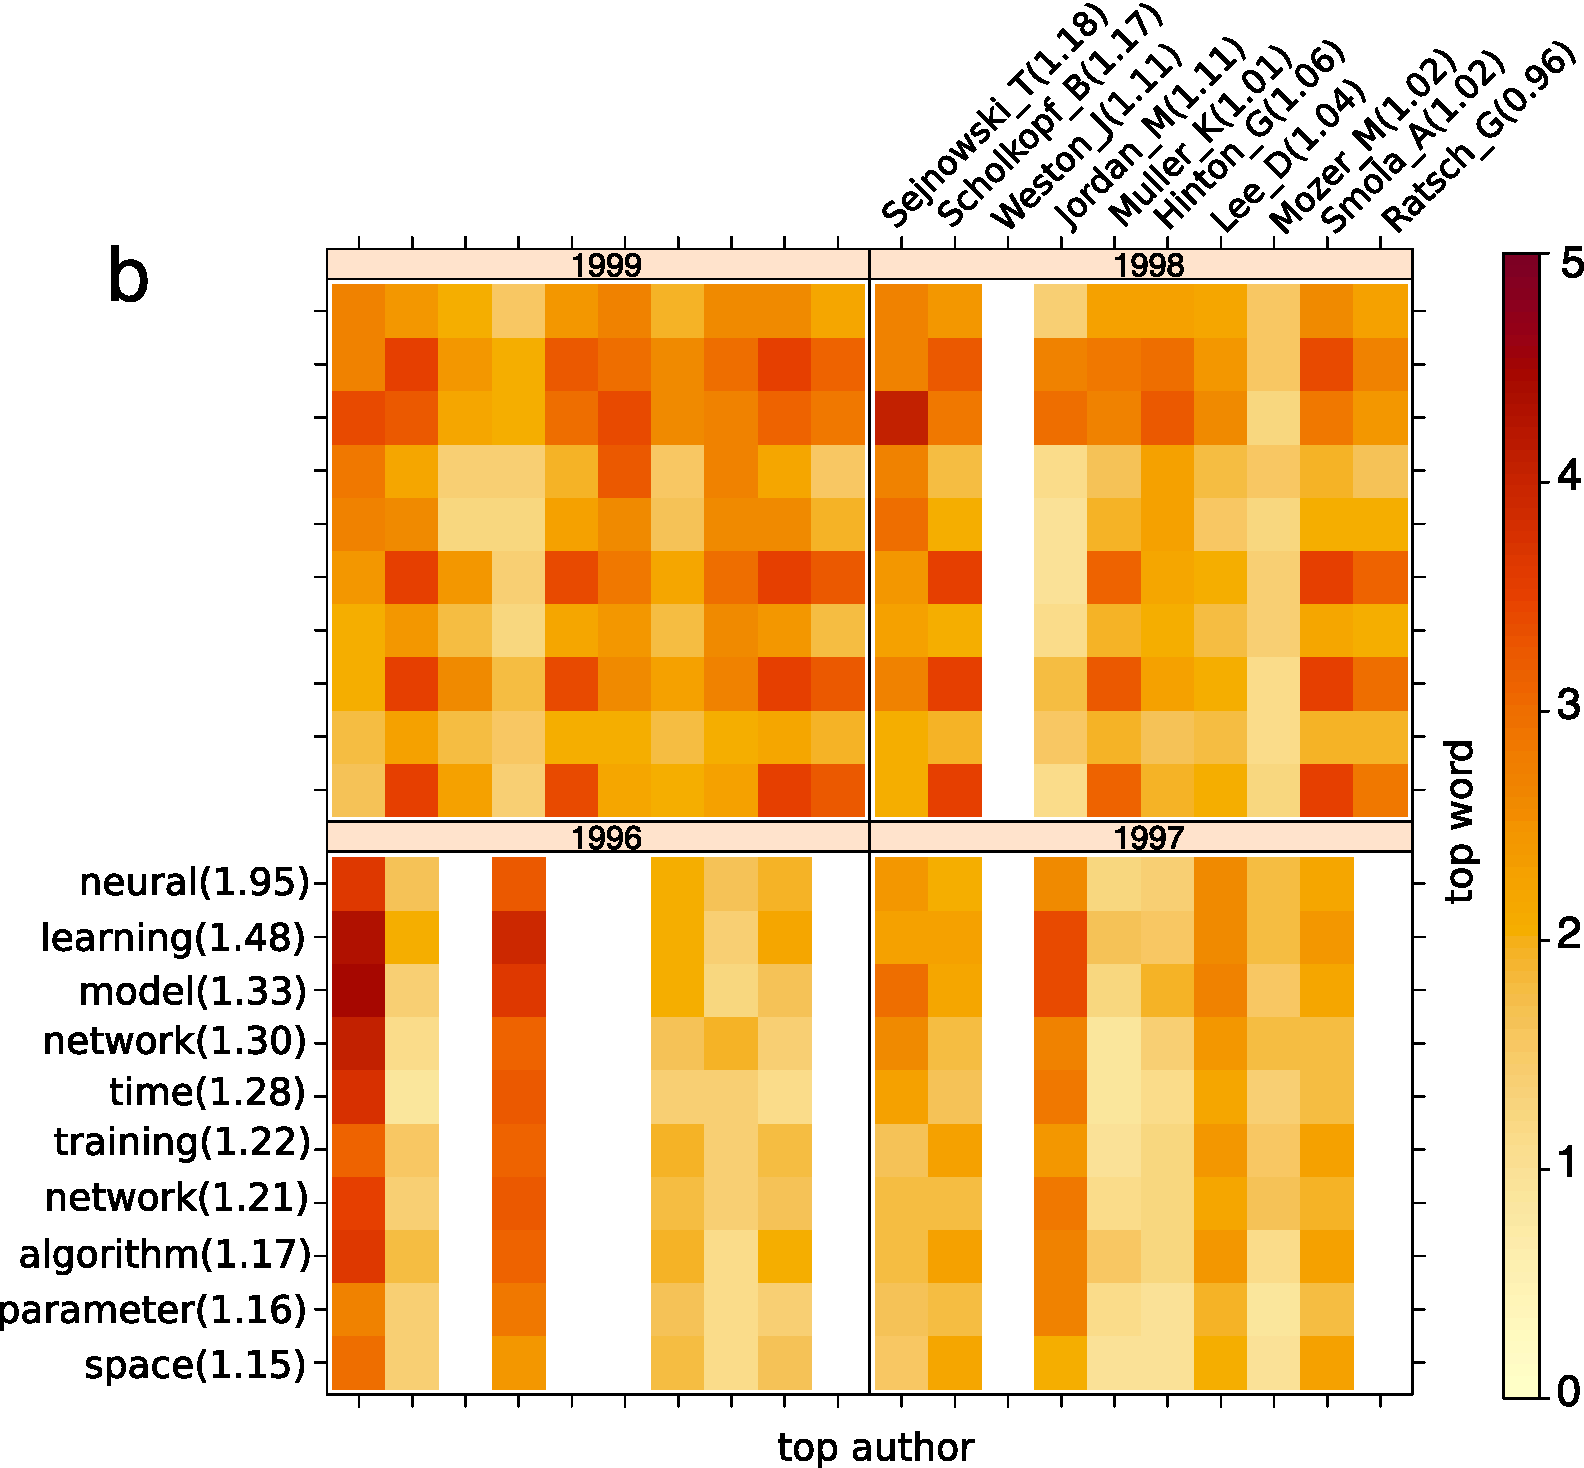
\includegraphics[width=.45\textwidth]{figure/signal.pdf}
 \captionsetup{justification=raggedright,font=small}
\caption{Estimated signal tensors in the data analysis. (a) top edges associated with IQ scores in the brain connectivity data. The color indicates the estimated IQ effect size. (b) top authors and words for years 1996-1999 in the NIPS data. Authors and words are ranked by marginal averages based on $\hat \Theta$, where the marginal average is denoted in the parentheses.
}\label{fig:signal}
\end{figure}




We next examine the estimated signal tensor $\hat \Theta$ from our method. Figure~\ref{fig:signal}a shows the results from brain connectivity dataset. We plot the top 10 brain edges based on regression analysis of denoised connection strengths against normalized IQ scores. We find that top connections are mostly inter-hemisphere edges, consistent with recent research on brain connectivity with intelligence~\citep{li2009brain,wang2017bayesian}. Figure~\ref{fig:signal}b illustrates the results from NIPS data, where we plot the entries in $\hat \Theta$ corresponding to top authors and most-frequent words (after excluding generic words such as \emph{figure}, \emph{results}, etc). The identified pattern is consistent with the active topics in the NIPS publication. Among the top words are \emph{neural} (marginal mean = 1.95), \emph{learning} (1.48), and \emph{network} (1.21), whereas top authors are \emph{T.\ Sejnowski} (1.18), \emph{B.~Scholkopf} (1.17), \emph{M.\ Jordan} (1.11), and \emph{G.\ Hinton} (1.06). We also find strong heterogeneity among word occurrences across authors and years. For example, \emph{training} and \emph{algorithm} are popular words for \emph{B.\ Scholkopf} and \emph{A.\ Smola} in 1998-1999, whereas \emph{model} occurs more often in \emph{M.\ Jordan} and in 1996. The detected pattern and achieved accuracy demonstrate the applicability of our method.

\section{Conclusion}
We have developed a tensor completion method that addresses both low- and high-rankness based on sign series representation. Our work provides a nonparametric framework for tensor estimation, and we obtain results  previously impossible. Applications to the brain connection data and topic data analysis yield conclusions with sensible interpretations, suggesting the practical utility of the proposed approach. Our work unlocks several possible future directions of nonparametric modeling of multi-task learning and compressed sensing. We hope the work opens up new inquiry that allows more researchers to contribute to this field.
\label{lastpage}

\newpage
\begingroup\footnotesize
\let\section\section
\makeatletter
%\renewcommand\@openbib@code{\itemsep\z@}
\makeatother
\bibliographystyle{chicago}
\bibliography{tensor_wang}
\endgroup



\end{document}
